\section{Theoretical Analysis}
\label{sec:analysis}
\paragraph{}
\par In this section, the circuit shown in Figure \ref{circuit} is analysed
theoretically, using the mesh method and the nodes method. The known values can be seen in the following table.
\begin{table}[H]
    \centering
    \begin{tabular}{|c|c|}
    \hline
        $R_1$ & 1.02362892933kOhm \\ \hline 
        $R_2$ & 2.08640382129kOhm \\ \hline
        $R_3$ & 3.09996108706kOhm \\ \hline
        $R_4$ & 4.08183334334kOhm \\ \hline
        $R_5$ & 3.0416957579kOhm  \\ \hline
        $R_6$ & 2.04156679366kOhm \\ \hline
        $R_7$ & 1.04156790057kOhm \\ \hline
        $V_a$ & 5.17885996884V \\ \hline
        $I_d$ & 1.04908336809mA \\ \hline
        $K_b$ & 7.29571922963mS \\ \hline
        $K_c$ & 8.16840649221kOhm \\ \hline	
    \end{tabular}
    \caption{Known Data}
    \label{data}
\end{table}
\subsection{Mesh Method}
\paragraph{}
\par To fully understand this particular method, the concept of mesh needs to be clarified. A mesh is a loop that contains no other loops. Then, it is possible to determine, via Kirchhoff Voltage Law (KVL), the current in each mesh. With that information, using Ohm's Law, it is possible to determine every voltage in the circuit, knowing the resistances in the mesh. This method requires an attentive observer that can identify meshes, therefore, is not often used in automation processes.

\par Firstly, four meshes were indentified in the circuit. The equations were writen and the flow of the current was stipulated, as can be seen in figure \ref{mesh}. 

\begin{figure}[H]
    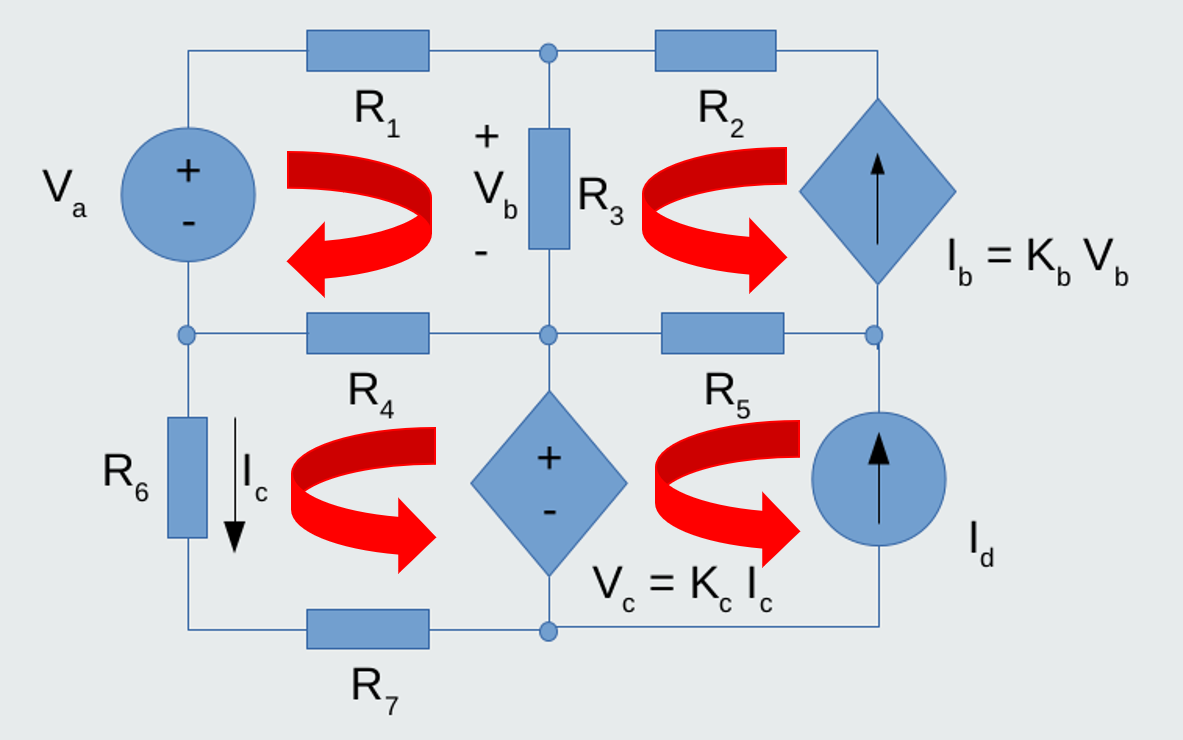
\includegraphics[width=0.5\linewidth]{Mesh.png}
    \centering
    \caption{Mesh Method applied to the circuit}
    \label{mesh}
\end{figure}

\par Simplifying the mesh method, the following system of equations \ref{system mesh} was writen. 
$$
\begin{cases} 
	V_a = R_{1}I_{a}+R_{3}(I_{a}+I_{b})+R_{4}(I_{a}+I_{c}) \\ 
	V_b = \frac{I_{b}}{K_{b}} = R_{3}(I_{a}+I_{b}) \\ 
	V_c = K_{c}I_{c} = R_{4}(I_{a}+I_{c})+R_{6}I_{c}+R_{7}I_{c}
\label{system mesh}
\end{cases}
$$


\par It was transformed into the following system \ref{matrix} and solved using the software \textit{Octave}. 

\begin{equation}
	\begin{bmatrix}
		R_1+R_3+R_4 & R_3 & R_4 & 0 \\
		R_4 & 0 & -K_c+R_4+R_6+R_7 & 0 \\
		R_3 & R_3-\frac{1}{K_b} & 0 & 0 \\
		0 & 0 & 0 & 1
	\end{bmatrix}
	\begin{bmatrix}
		I_a     \\
		I_b     \\
		I_c \\
		I_d     \\
	\end{bmatrix}
    =
	\begin{bmatrix}
		V_a     \\
		0     \\
		0  \\
		0     \\
	\end{bmatrix}
	\label{matrix}
\end{equation}

\par Therefore, the values for the voltage and current sources were determined and can be seen in the following table \ref{results mesh}, being the unit for current mA and the unit for voltage V. 

\begin{table}[H]
    \centering
    \begin{tabular}{|c|c|}
    \hline
        $I_a$ & 2.401364132117077e-01 \\ \hline 
        $I_b$ & 2.512453816512571e-01 \\ \hline
        $I_c$ & 9.768380052260230e-01 \\ \hline
        $I_d$ & 1.049083368090000e+00 \\ \hline
        $V_a$ & 5.178859968840000 \\ \hline
        $V_b$ & 3.443736987998083e-02 \\ \hline
        $V_c$ & 7.979209903725712\\ \hline
    \end{tabular}
    \caption{Table of results for the mesh method}
    \label{results mesh}
\end{table}

\subsection{Node Method}
\paragraph{}
\par Nodes are any regions between any two elements of the circuit. With Kirchhoff Current Law (KCL) it is possible to determine any nodal voltage. The KCL cannot be used in nodes that are connected to a voltage source. This means those nodes must have relations with the source, making it possible to solve the system. In opposition to the mesh method, this method is easy to automate due to its methodical approach, being possible to extract values in a simulation very easily.
The first approach is to name every node so it is possible to start the analysis.


\par First, the nodes were represented in the circuit as can be seen in figure \ref{circuitlt}. The software used to represent the circuit and to provide another simulation to confirm the one explained on \ref{sec:simulation} was \textit{LTSpice}.

\begin{figure}[H]
    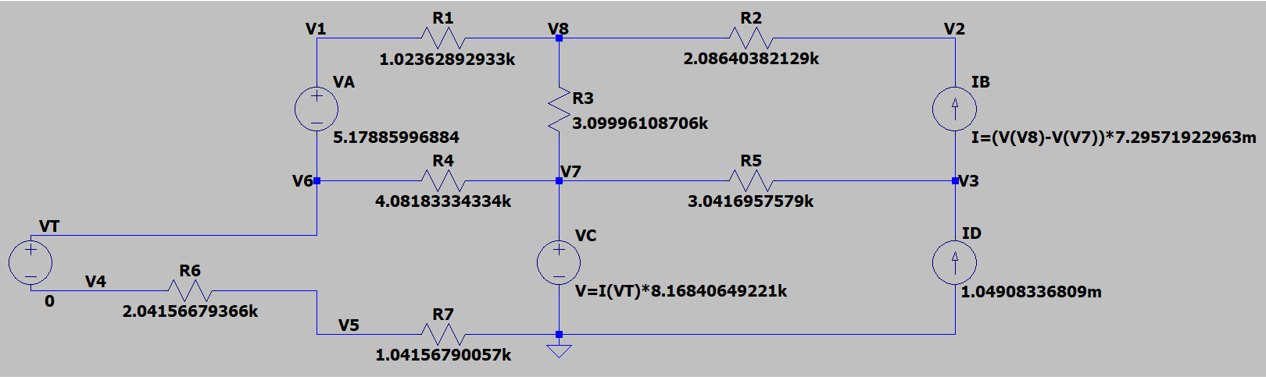
\includegraphics[width=0.8\linewidth]{CircuitLTSpice.png}
    \centering
    \caption{Circuit represented through \textit{LTSpice}}
    \label{circuitlt}
\end{figure}


\par Then, the equations for the nodes method were writen according to the numeration visible in the circuit above. The voltage source $V_T$ was created to help in the simulation analysis, the reason behind it will be explained later.
$$
\begin{cases} 
	V_1 - V_6 = V_a \\ 
	\frac{V_2 - V_8}{R_2} - K_b*(V_8 - V_7) = 0 \\
	-I_d + \frac{V_3 - V_7}{R_5} + K_{b}(V_8 - V_7) = 0 \\ 
	\frac{V_5 - V_6}{R_6} + \frac{V_5}{R_7} = 0 \\
	\frac{V_8 - V_1}{R_1} + \frac{V_8 - V_2}{R_2} - \frac{V_8 - V_7}{R_3}  = 0 \\
	\frac{V_6 - V_7}{R_4} + \frac{V_6 - V_5}{R_6} - \frac{V_1 - V_8}{R_1}  = 0 \\
	V_7 = -K_c \frac{V_5 - V_6}{R_6}
\label{system nodes}
\end{cases}
$$
\par The equations above were transformed into the following system \ref{matrixn} so that \textit{Octave} could solve it.
\begin{equation}
	\begin{bmatrix}
		1 & 0 & 0 & 0 &-1 & 0 & 0 \\
		0 & \frac{1}{R_2} & 0 & 0 & 0 & K_b & \frac{-1}{R_2}-K_b \\
		0 & 0 & \frac{1}{R_5} & 0 & 0 & \frac{-1}{R_5}-K_b & K_b \\
		0 & 0 & 0 & \frac{1}{R_6}+\frac{1}{R_7} & \frac{-1}{R_6} & 0 & 0 \\
		\frac{-1}{R_1} & \frac{-1}{R_2} & 0 & 0 & 0 & \frac{-1}{R_3} & \frac{1}{R_1}+\frac{1}{R_2}+\frac{1}{R_3} \\
		\frac{1}{R_1} & 0 & 0 & \frac{-1}{R_6} & \frac{1}{R_4}+\frac{1}{R_6} & \frac{-1}{R_4} & \frac{-1}{R_1} \\
		0 & 0 & 0 & \frac{K_c}{R_6} & \frac{-K_c}{R_6} & 1 & 0]
	\end{bmatrix}
	\begin{bmatrix}
		V_1     \\
		V_2     \\
		V_3  \\
		V_5  \\
		V_6   \\
		V_7   \\ 
		V_8     \\
	\end{bmatrix}
    =
	\begin{bmatrix}
		V_a     \\
		0     \\
		I_d  \\
		0     \\
		0     \\
		0     \\
		0     \\
	\end{bmatrix}
	\label{matrixn}
\end{equation}

\par Hence, the values for the current sources and the voltage in each point $V_1$ to $V_8$ were calculated and can be seen in the table below, again being the unit for current mA and the unit for voltage V. $V_4$ is only in the circuit for simulation purposes, with voltage equal to $V_6$, $V_4$ is supressed in the analysis.

\begin{table}[H]
    \centering
    \begin{tabular}{|c|c|}
    \hline
        $V_1$ & 8.190583113394776e+00\\ \hline
        $V_2$ & 7.420573209487090e+00\\ \hline
        $V_3$ & 1.193441434568911e+01\\ \hline
        $V_5$ & 1.017443110300255e+00\\ \hline
        $V_6$ & 3.011723144554777e+00\\ \hline
        $V_7$ & 7.979209903725710e+00\\ \hline
        $V_8$ & 7.944772533845730e+00\\ \hline
        $I_a$ & 2.401364132117075e-01\\ \hline 
        $I_b$ & 2.512453816512545e-01\\ \hline
        $I_c$ & 9.768380052260227e-01\\ \hline
        $I_d$ & 1.049083368090000e+00\\ \hline
    \end{tabular}
    \caption{Table of results for the node method}
    \label{results node}
\end{table}

\par Using
\begin{equation}
	V_b=\frac{I_b}{K_b}
\label{Vb}
\end{equation}
and
\begin{equation}
	V_c=K_{c}I_{c}
\end{equation}
one can get the following results:
\begin{table}[H]
    \centering
    \begin{tabular}{|c|c|}
    \hline
        $V_a$ & 5.178859968840000\\ \hline
        $V_b$ & 3.443736987998047e-02\\ \hline
        $V_c$ & 7.979209903725709\\ \hline
    \end{tabular}
    \caption{Values of $V_a$, $V_b$ and $V_c$}
\end{table}

\par It is evident that the two methods return values with notorious resemblance.

\par The simulation, explained on the next section, will be compared with the two theoretichal analysis in order to identify any incompability with the theory, allowing further discussion.
